\documentclass[10pt]{article}

%\newif\ifpdf
%\ifx\pdfoutput\undefined
%\pdffalse % we are not running PDFLaTeX
%\else
%\pdfoutput=1 % we are running PDFLaTeX
%\pdftrue
%\fi

%\ifpdf
%\usepackage[pdftex,bookmarksnumbered,colorlinks,backref, bookmarks, breaklinks, linktocpage]{hyperref}
%\else
%\usepackage[dvips,bookmarksnumbered,colorlinks,backref, bookmarks, breaklinks, linktocpage]{hyperref}
%\fi

%\usepackage{algorithm,algorithmic}
\usepackage{graphicx}
%\usepackage{fancyhdr}
\usepackage{subfigure}
%\usepackage{url}
%\usepackage{hyperref}

%\bibliographystyle{unsrt}
\usepackage{mathtools}
\usepackage{amsmath}
\usepackage{amsfonts}
\usepackage{amssymb}
\usepackage{calligra}
\DeclareMathAlphabet{\mathcalligra}{T1}{calligra}{m}{n}

%%% Notations
\newcommand{\wrt}{w.\,r.\,t.}
\newcommand{\eg}{e.\,g.}
\newcommand{\ie}{i.\,e.}
\newcommand{\Ie}{I.\,e.}
\newcommand{\Dash}{\nobreak\,---\penalty-500\,}
%\newcommand{\Dash}{\nobreak\,---\,}
\newcommand{\mystrut}{\vrule height2.5ex depth.2ex width0pt}
\DeclareMathAlphabet{\mathbi}{T1}{cmr}{bx}{it}
\newcommand{\stat}{{\mathbi{s}}}
\newcommand{\x}{{\mathbi{x}}}
\newcommand{\y}{{\mathbi{y}}}
\newcommand{\ds}{{\mathbi{d}}}
\newcommand{\op}{$\mathcal{O}$}

\newcommand{\Model}{\mathcal{M}}
\newcommand{\State}{\mathbf{s}}
\newcommand{\Params}{\mathbf{p}}
\newcommand{\Control}{\mathbf{c}}


\newcommand{\sstate}{\textit{{S-state}}}
\newcommand{\mstate}{\textit{{M-state}}}
\newcommand{\ssda}{\textit{SSDA}}

\newcommand{\smp}{$\sigma-$\textit{point}}

%%% Optimus components
\newcommand{\al}{\texttt{FilteringAnimationLoop}}
\newcommand{\ssw}{\texttt{StochasticStateWrapper}}
\newcommand{\psw}{\texttt{PreStochasticWrapper}}
\newcommand{\ukf}{\texttt{UKFilter}}
\newcommand{\roukf}{\texttt{ROUKFilter}}
\newcommand{\ukfsc}{\texttt{UKFilterSimCorr}}
\newcommand{\etkf}{\texttt{ETKFilter}}
\newcommand{\opr}{\texttt{OptimParams}}
\newcommand{\mobs}{\texttt{MappedStateObservationManager}}


\setlength{\topmargin}{1cm}
\setlength{\oddsidemargin}{1cm}
\setlength{\textheight}{21.0cm}
\setlength{\textwidth}{15cm}



%\renewcommand{\chaptermark}[1]% 
%	{\markboth{{\thechapter.\ #1}}{}} 
%\renewcommand{\sectionmark}[1]% 
%	{\markright{{\thesection.\ #1}}} 
%\renewcommand{\headrulewidth}{0.5pt} 
%\renewcommand{\footrulewidth}{0pt} 
%\newcommand{\helv}{% 
%	\fontfamily{phv}\fontseries{b}\fontsize{9}{11}\selectfont} 
%\fancyhf{} 
%\fancyhead[LE,RO]{\thepage} 
%\fancyhead[LO]{\rightmark} 
%\fancyhead[RE]{\leftmark}

\begin{document}

\section{Data Assimilation and State Estimation in SOFA}
\label{s:overview}
Optimus plugin was created to provide a testing environment for data-driven physics-based modeling (typically finite elements, FE).
While actually the plugin implements only stochastic methods based on Kalman filtering, its architecture allows for implementation of 
generic prediction--correction schemes where the model is employed as a predictor and correction is performed using given observation data. 

In this text, a model $\Model$ performs a transformation of state $\State$ given parameters $\Params$ and control $\Control$, \ie, 
\begin{equation}
\State \xrightarrow{\Model(\Params, \Control)} \State'.
\end{equation}
Typically, the model is represented by SOFA components such as force fields. The state is given by positions and optionally velocities, and
control is provided as applied forces, pressures and/or prescribed displacements. Parameters are given by the type of model; typically, these are
mechanical parameters (Young's modulus, spring stiffness). 

It is assumed that one or combination of following types of estimation is performed:
\begin{itemize}
	\item {\bf State estimation:} typical scenario in Kalman filtering where the state $\State$ of the model is assumed to suffer from uncertainties due to 
	the initial conditions (\ie, the state at time $t_0$) and/or modeling itself. The correction aims at improving the estimation of the state given the observations.
	\item {\bf Parameter identification:} this scenario is usually known as \emph{data assimilation}: the main source of uncertainty is related to the 
	parameters of the model, \ie, uncertanty related to the stiffness of an organ. The goal is thus to \emph{learn} the actual value of the parameter(s)
	given the observations. 
	\item {\bf Joint state--parameter estimation:} while the parameters are source of uncertainty, even a perfect  knowledge of the parameters does not 
	provide completely reliable results since the model itself (even if accurately parametrized) is imperfect, and/or there is an inherent uncertainty 
	related to the initial conditions. 	
\end{itemize}
Recently, in the context of estimation of boundary conditions, we have been interested in {\bf control estimation}, for example, estimation of applied forces. 
To summarize, Optimus plugin allows for estimation or identification of any quantity that can be \emph{delivered} to a SOFA component. either through a data engine (parameters, forces) or via write accessors (positions, velocities).


\subsection{State handling and animation loop}
Adopting the naming conventions in both the mechanics and filtering, we end up with two notions of states:
\begin{description}
	\item[Mechanical state:] Configuration of the object being simulated, typically given by positions and velocities. This state is always deterministic, \ie\, it is represented by a single vector of mechanical degrees of freedom (DoFs). This state is typed using SOFA types (Vec3d, Rigid3d and similar). 
	In this text, mechanical state is abbreviated as \mstate.
	\item[Stochastic state:] Quantity given as a probability distribution (PD), represented by its statistics. In case of Gaussian PD considered here, the statistics are the expected value and the standard deviation. From the physical point of view, this state may contain an arbitrary combination of positions, velocities, parameters and forces. It is stored a set of Eigen vectors (e.g., two of them for Gaussian PD). In this text, stochastic state is abbreviated as \sstate.
\end{description}
In Optimus, \mstate\ is strictly separated from \sstate both conceptually and from the implementation point of view and these two terms cannot be interchanged. While the filter works {\bf only} with \sstate, classical SOFA components (e.g. components from SOFA framework and other existing plugins) employ only \mstate. The interface between \sstate\ and \mstate is provided by the \ssw\ and \opr\ components.



\section{Data Assimilation description}

%{\large\bf Initially, Optimus plugin was based on Verdandi library. The concepts remain very similar: mainly, the Verdandi-related stuff has been replaced by SOFA-filtering (as explained above).}

\subsection{Parameter handling}
The main goal of the stochastic state data assimilation (\ssda)\ (and data assimilation in general) is to estimate a set of model parameters based on the model dynamics and observations,
where both are associated with uncertainties.

From the SOFA point of view, the parameters are usually simple numbers (or vectors of numbers) handled by local components: for example, the Young's modulus is a number (usually constant) defined and handled by the FEM-component, stiffnesses of a set of springs is a vector handled by the spring component.

However, in estimation process, the parameters are included in the extended  state (\sstate\ in our case) and they evolve together with the model state. The parameters are not regarded as simple numbers, but as probability distributions (defined by corresponding statistics as mean value and variance). Since the model itself requires concrete instances the parameters, these are instantiated in each \texttt{Forward} step using the method of \smp.

In order to integrate the two different concepts, a new component was introduced, namely \opr:
\begin{itemize}
\item The component is a container of parameters which vary during the \ssda. The parameters are defined using \emph{initial value} and \emph{standard deviation}.
\item It also handles correct update of the \sstate: it works as an \emph{interface} between SOFA and Filtering components. 
\item If option \texttt{optimize} is true (which is the case by default), \textbf{the node containing the component is considered as the part of the physical model assimilated by filtering process}. If in a node this component is not present, or \texttt{optimize="0"}, the object modeled by the node is not included in the assimilation.
\end{itemize}
In each phase and step of the \ssda, the actual value of the parameters handled by \opr\ can be accessed via SOFA \texttt{Data<> value}. Therefore, the components which depends on the parameters being optimized (such as already mentioned Young's modulus) must be linked via @. \textbf{It must be verified, that the component which depends on the parameters being optimized is compatible with the fact that this parameter changes in each step,} \ie\ there are no internal structures which are precomputed using the initial values of the parameters.

The \opr\ component was conceived to be as general as possible, therefore it can handle structures defined as \texttt{Data<DataTypes>} where \texttt{DataTypes} is the parameter of template (which could be virtually any type (scalars, vectors of scalars, \emph{VecCoord} etc.). In order to achieve this degree of generality, the concept of \emph{functors} was employed as can be seen in the code of the component.

Finally, in one node, several  \opr\ can be present if different types of parameters are to be optimized (this has been test only partially\ldots).

\subsection{Prediction: \texttt{Forward}}
In the forward stage, the filter performs the prediction phase by evaluating on \emph{operator} (UKF) and/or it's derivatives (EKF). This evaluation
is done for each \smp\ independently and the 
result is used to compute the mean prediction (\emph{a priori}) value of the \sstate. The \emph{operator} \op\ is in fact a time step of the model,
here represented by a standard SOFA simulation time step.
A few facts about \op\ must be emphasized:
\begin{itemize}
\item From the filtering context, it acts on the state (\sstate), so for a given \sstate\ $X_n$ it performs $X^-_{n+1} =
\mathcal{O}(X_{n})$.  
\item From the SOFA point of view, it performs a single step of the simulation on a given DoF positions/velocities (encoded as a part of $X_n$)  while
taking into account the current parameters (also encoded as a part of $X_n$).
\item It is evaluated several times in each step of \ssda, namely, it is evaluated for each \smp\ which is a different perturbation of $X_{n+1}$
according to the chosen method (simplex, star, circle). 
\end{itemize}

In order to facilitate the integration with SOFA, it was desirable to make the real evaluation of \op\ (SOFA model) completely transparent
from the filtering process. 
For this reason, a new component \ssw\  was created: it serves as a wrapper of all physical simulation components and ensures the correspondence between the respective mechanical states and the \sstate.

This part is also the trickiest one in terms of the implementation as the SOFA components are usually not implemented with the idea of total independence on the software.

The forward stage is computationally  expensive mainly due to multiple evaluation of the model; the subsequent manipulation with \sstate\ are rather cheap. At the same time, the execution of the operator is embarrassingly parallel. However, the main issue is that for a parallelization on $N$ threads, $N$ independent copies of the SOFA world would have to be created.


\subsection{Correction: \texttt{Analyze}}
While the forward stage requires a significant manipulation of \sstate\ and simulation components, analyze stage is almost exclusively performed by filter. The only part supplied by SOFA is the \texttt{ObservationManager} which computes an \emph{innovation} using prediction computed previously and observations obtained by an external source.

So far, we have been experimenting only with simple cases where the observations are generated using a \emph{forward simulation}, \ie\ a standard SOFA simulation where the states of the modeled objects are stored in each step into a text file using SOFA monitors. Then, each simulation scene has to have an \emph{observation sub-node} which contains following components:
\begin{itemize}
\item Mechanical object which defines a set of observation points. These can be any points inside the moving objects were observations are made (trivially, it can be equivalent to the mechanical 
state of the assimilated object).
\item Mapping between the observation mechanical state and the mechanical state of the assimilated body (trivially an \texttt{IdentityMapping}, usually a \texttt{BarycentricMapping}).
\item An observation manager which provides a method \texttt{GetInnovation} called by the filter. The method must have an access to observation in each time (supplied for example by an \texttt{ObservationSource} and it uses mapping (\texttt{Apply}) to get the observations in points
defined by the mechanical state. 
\end{itemize}

So far we are using \texttt{SimulationStateObservationSource} in order to read the positions exported by monitors in forward simulations. Currently, the code allows for adding a noise, although only in very preliminary version.



\section{Components}
{\large \al}
\begin{itemize}
\item Compliant with SOFA API for animation loops. 
\item Calls filter wrapper to perform the assimilation in each step.
\item Issues special events: PredictionEndEvent after calling the prediction step of the filter, and CorrectionEndEvent after calling the correction step of the filter.
\end{itemize}
\medskip
{\large\ssw}
\begin{itemize}
\item Wrapper of model provided by SOFA. This wrapper implements the interface between the stochastic components (filters) and SOFA simulation.
\item Must be placed inside the SOFA subnode containing the physical simulation components.
\item Requires MechanicalObject and assumes OptimParams in the same node.
\end{itemize}
\medskip
{\large\psw}
\begin{itemize}
\item Special version of wrapper which allows for including other simulated object into Optimus scene which do not contain any quantities being estimated.
\item Typical example is an obstacle which displays a physical behaviour, however, none of its features is directly involved in the estimation.
\end{itemize}
\medskip
{\large \ukf}
\begin{itemize}
\item Unscented Kalman Filter proposed by Julier and Uhlman (1997)~\cite{JulierUnscentedKF1995, JulierKalmanFExtension1997}.
\item Main methods are initializeStep(), computePrediction() and computeCorrection(), all called by the \al.
\end{itemize}
\medskip
{\large \roukf}
\begin{itemize}
\item Reduced order Kalman filter implemented according to Moireau, Philippe, and Dominique Chapelle~\cite{MoireauReducedOrder2011}.
\item Main methods are initializeStep(), computePrediction() and computeCorrection(), all called by the \al.
\end{itemize}
\medskip
{\large \ukfsc}
\begin{itemize}
\item Special version of UKF filter purely for data assimilation~\cite{EbrahimianExtendedKalmanFilterForMaterialParameterEstimationInNonlinearStructuralFiniteElementModels2015}.
\item Main methods are initializeStep(), computePrediction() and computeCorrection(), all called by the \al.
\end{itemize}
\medskip
{\large \entkf}
\begin{itemize}
\item Ensemble Transform Kalman filter described in~\cite{HuttDivergenceOfTheEnsembleTransformKalmanFilter2020}. Instead of sigma points the transformation are performed with Ensemble members.
\item Main methods are initializeStep(), computePrediction() and computeCorrection(), all called by the \al.
\end{itemize}
\medskip
{\large\mobs}
\begin{itemize}
\item One instance of observation manager which handles the observations and provides them to the filter via computation of innovation.
\item Assumes that the predicted observations are mapped to the main mechanical object (associated with \ssw).
\item Templated on \texttt{DataTypes1} and \texttt{DataTypes2} since it calls mapping apply (having also two template parameters).
\item Inherits from \texttt{ObservationManager} which is only an abstract base.
\item The uncertainty of the observations is set using option \texttt{observationStdev} which is the standard deviation of observations assumed in the data assimilation.
\item Noise can be added using \texttt{noiseStdev}: the noise is generated using \texttt{Boost}, has a normal distribution with zero mean and standard deviation given by \texttt{noiseStdev}.
\end{itemize}
\medskip
{\large\opr}
\begin{itemize}
\item Container of Gaussian stochastic variables given by expected value and standard deviation.
\item Templated on any numerical type in SOFA, specializations needed.
\item Abstract pure base \texttt{OptimParamsBase} created to facilitate the manipulation and define the API.
\item In \emph{forward mode}, it can be used either as a simple container of parameters which remain constant, or as a \emph{parameter controller} which can change 
the parameters during the simulation. The change is defined using option \texttt{prescribedParamKeys="T$^0$ v$_0^0$ ... v$_n^0$  T$^1$ v$_0^1$ ... v$_n^1$ ... ... T$^t$ v$^t_0$ ... v$^t_n$"} where the 
values of parameters are defined in each time T$^t$ (not a time step, but the simulation time). Here, the option \texttt{numParams} is required in order to parse the keys correctly. 
The transition between two different values can be done smoothly (based on \texttt{tanh}), the option \texttt{interpolateSmooth}.
Finally, the initial value in the XML  file is ignored and only the keys are used so that the 
real value of the parameter is interpolated for given time step.
\item The value of parameteres in each time step can be exported using option \texttt{exportParamFile}.
\item In the \emph{filtering mode}, only the initial value \texttt{initValue} together with the standard deviation \texttt{stdev} are set in the XML file.
\item In some optimization cases, it's desirable to keep some properties of the parameters being optimized (e.g positivity for the Young's modulus. The option \texttt{transformParams} can be used to choose between: 0 the no transformation is done, 1: absolute value of the parameters is taken, before feeding the model. 2: sigmoid transformation of the parameters is taken, before feeding the model. 3: exponential transformation of the parameters is taken, before feeding the model. 4: projection of the parameters to the bounded space is taken, before feeding the model. The bounds of the projected space are defined using \texttt{minValue} and \texttt{maxValue} fields.
\end{itemize}
\medskip
{\large\texttt{SimulatedStateObservationSource}}
\begin{itemize}
\item Auxiliary components that reads and provides observations stored in a monitor file generated by a forward simulation.
\item Mainly supplies \texttt{GetObservation} method called by the observation manager. 
\item Requires correct prefix of the monitor-generated file. 
\end{itemize}



\section{Data}

The plugin contains several volume (VTK) and surface (STL) meshes used in the examples, benchmarks and scenes. Most of meshes were generated by GMesh generator.



\section{Visualization}

Optimus plugin has several python scripts that allow to show the dynamics of estimated parameters (stiffnesses), variance values, and correlation between parameters. All scripts use Matplotlib python library to draw figures and charts and YAML configuration files to load main scene parameters.

All visualization scripts are stored in python\_src/visualisation subfolder in Optimus. To scripts generally require only path to output folder(s) with results, since special subfolders structure, which is recognized by scripts, is generated and YAML is copied to output folder during data assimilation process.



\section{Examples}

{\large\bf This is a description of an old examples, which are now replaced by anothers.}

\subsection{EX1: Estimation of constant Young's moduli of segments of a heterogeneous object under gravity}

The data are generated using \texttt{CylinderModulusForward.scn} and in each step, the entire mechanical object of the cylinder is saved by the
\texttt{Monitor} component.
The cylinder is divided into three parts and each one is assigned different Young's modulus using OptimParams  (which are here used exclusively as a
container).

Data assimilation is performed by \texttt{CylinderModulusROUKF.scn} so that:
\begin{itemize}
 \item The observations are read from the file generated by \texttt{Monitor} in the forward simulation. 
 \item Either all DoFs can be used directly as observations (then \texttt{BarycentricMapping} is replaced by the \texttt{IdentityMapping}), or 
 a subset of points inside the cylinder are chosen as the observation points mapped to the cylinder via \texttt{BarycentricMapping}.
 \item The variance of error is set via \texttt{observationStdev} which is the standard deviation of the observation error which is the measure of the
uncertainty in observations. Note: zero cannot be used as the co-variance matrix cannot be inverted in this case.
 \item A white Gaussian noise can be added to the observations via the option \texttt{noiseStdev}. In general, \texttt{observationStdev} should be
equal to \texttt{noiseStdev}: we use two separated options for experimental purposes.
 \item The initial values of the estimated parameters together with initial standard deviation is set in \texttt{OptimParams}.
 \item The vector of the actual estimations of the parameters can be stored at the end of each step using a non-empty filename \texttt{paramFileName}
and the variance matrix is stored in a vectorial 
 form using a non-empty filename \texttt{paramVarFileName}: first the diagonal, then off-diagonal elements under and above the diagonal, respectively
(which is redundant as the matrix is symmetric). 
 \end{itemize}
 

 Visualization:
 \begin{itemize}
  \item Cylinder: different colors associated to different Young's moduli. 
  \item Red points: the actual position of the observation points on the model with estimated parameters  
  \item Blue points: the actual position of the observation points loaded from the \texttt{Monitor} file with added noise.
 \end{itemize}
 

Several examples of the assimilation are given below for different settings in the data-assimilation scene, showing the evolution of the parameter
estimation and the variance (standard deviation squared) of the 
parameters.


\begin{figure}[ht]
\begin{center}
%\subfigure[]{
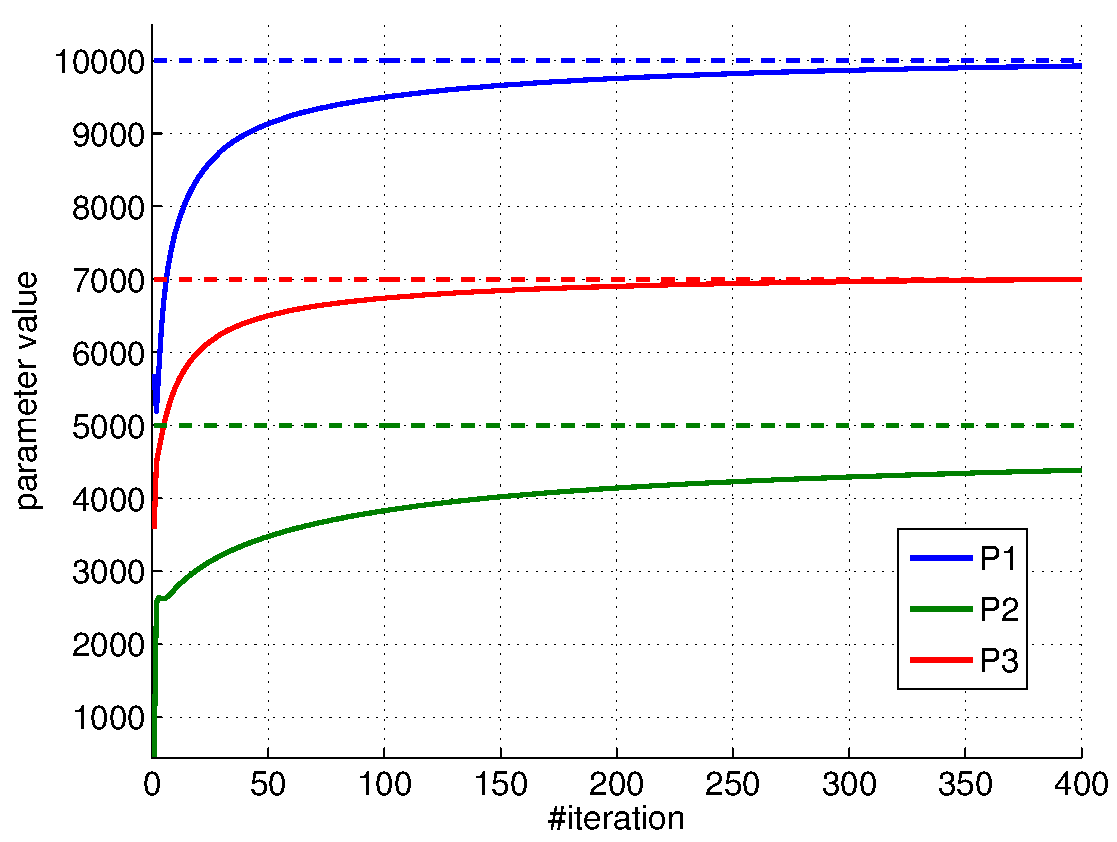
\includegraphics[width=.49\linewidth]{figures/p1_estim.pdf}
\hfill
%\subfigure[]{
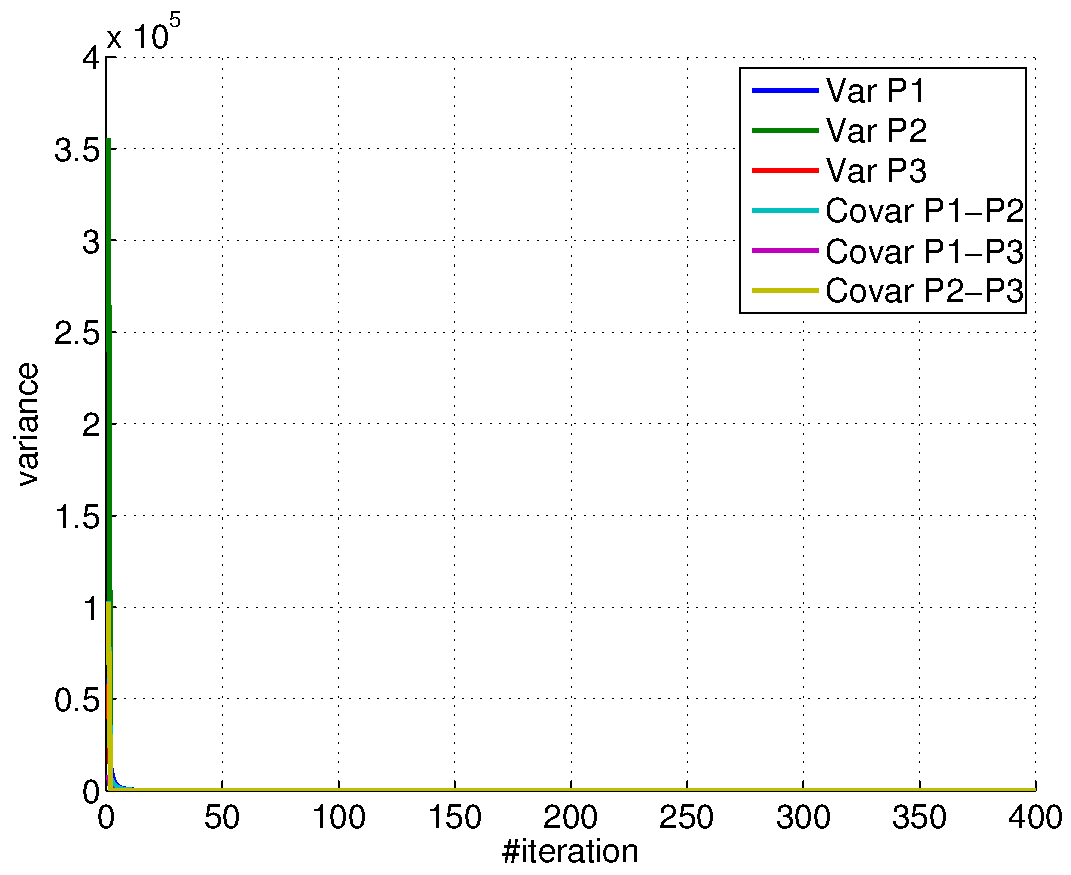
\includegraphics[width=.49\linewidth]{figures/p1_var.pdf}
\caption{Parameters: \texttt{initValue="6000"}, \texttt{stdev="2000"}. Observations: all DoFs (3$\times$number of mesh nodes),
\texttt{observationStdev=1e-4} no noise added. A naive scenario, where everything is known and no uncertainty exists.}
\label{fig:Results1}
\end{center}
\end{figure}


\begin{figure}[ht]
\begin{center}
%\subfigure[]{
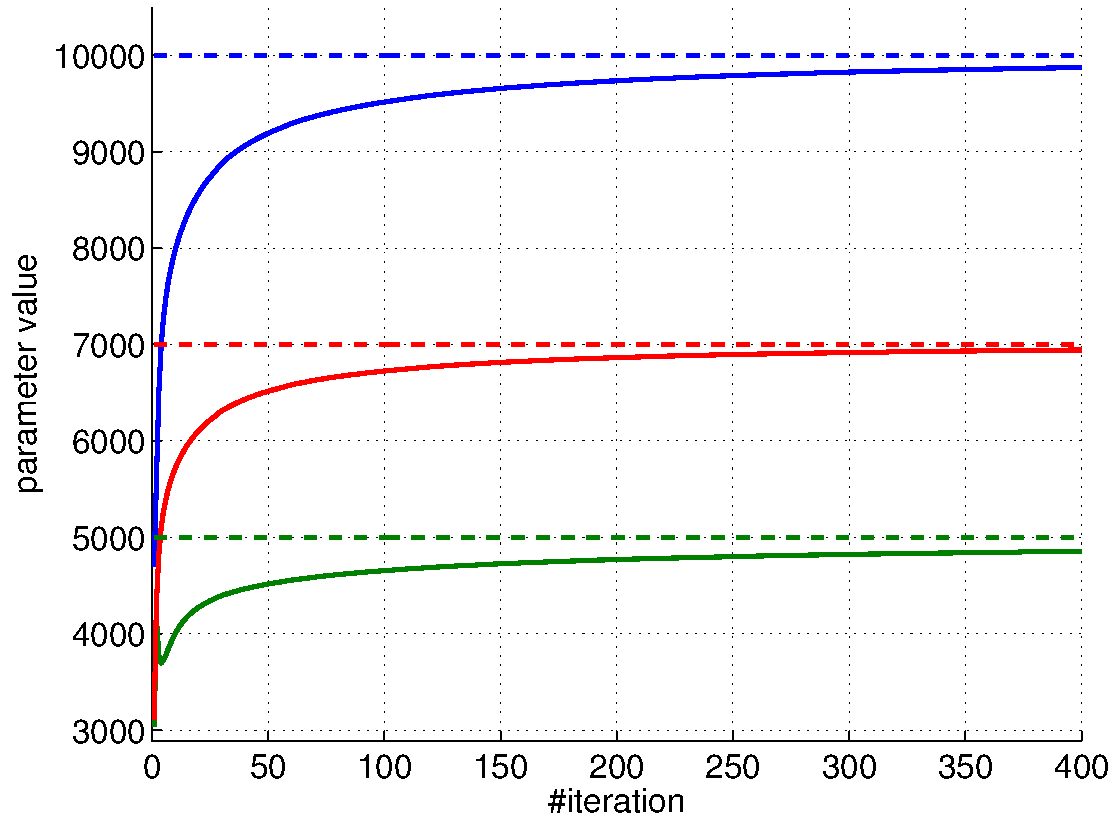
\includegraphics[width=.49\linewidth]{figures/p2_estim.pdf}
\hfill
%\subfigure[]{
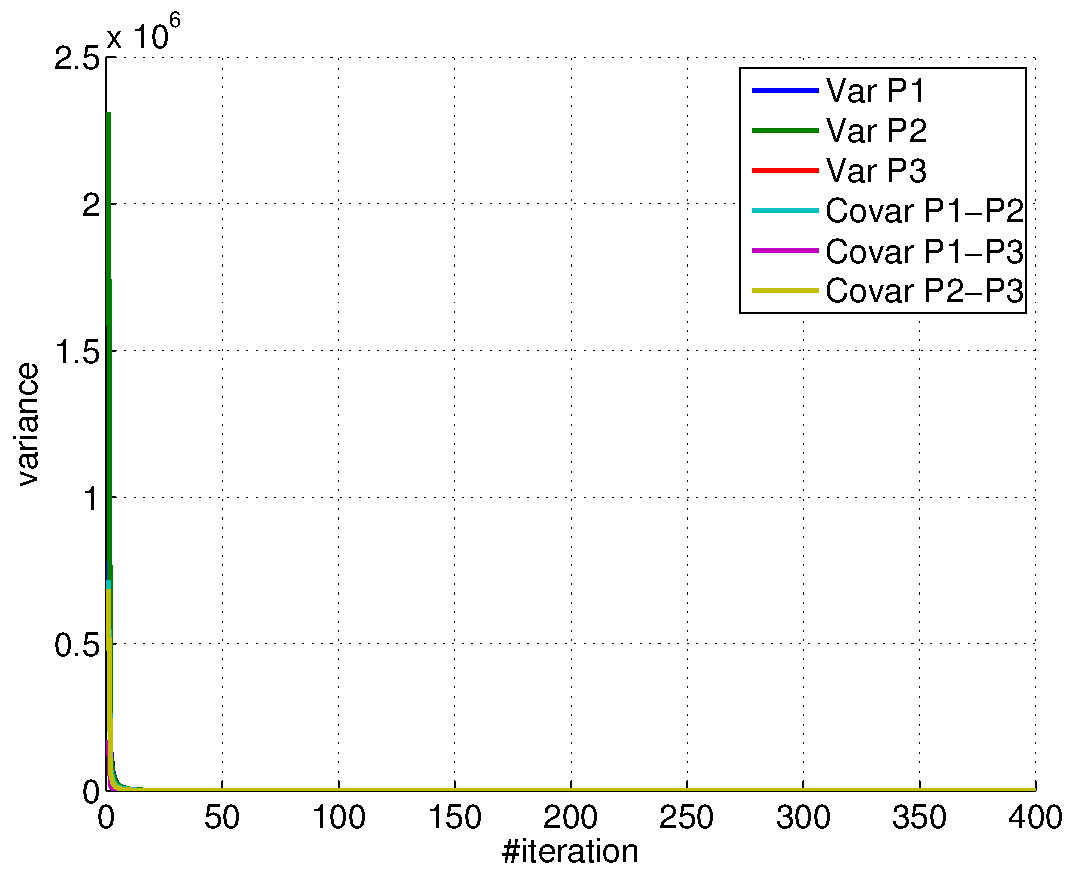
\includegraphics[width=.49\linewidth]{figures/p2_var.pdf}
\caption{Parameters: \texttt{initValue="6000"}, \texttt{stdev="2000"}. Observations: 10 points selected along the centerline,
\texttt{observationStdev=1e-4} no noise added. Still quite naive scenario, where number of observations is limited, but still no uncertainty exists.}
\label{fig:Results2}
\end{center}
\end{figure}



\begin{figure}[ht]
\begin{center}
%\subfigure[]{
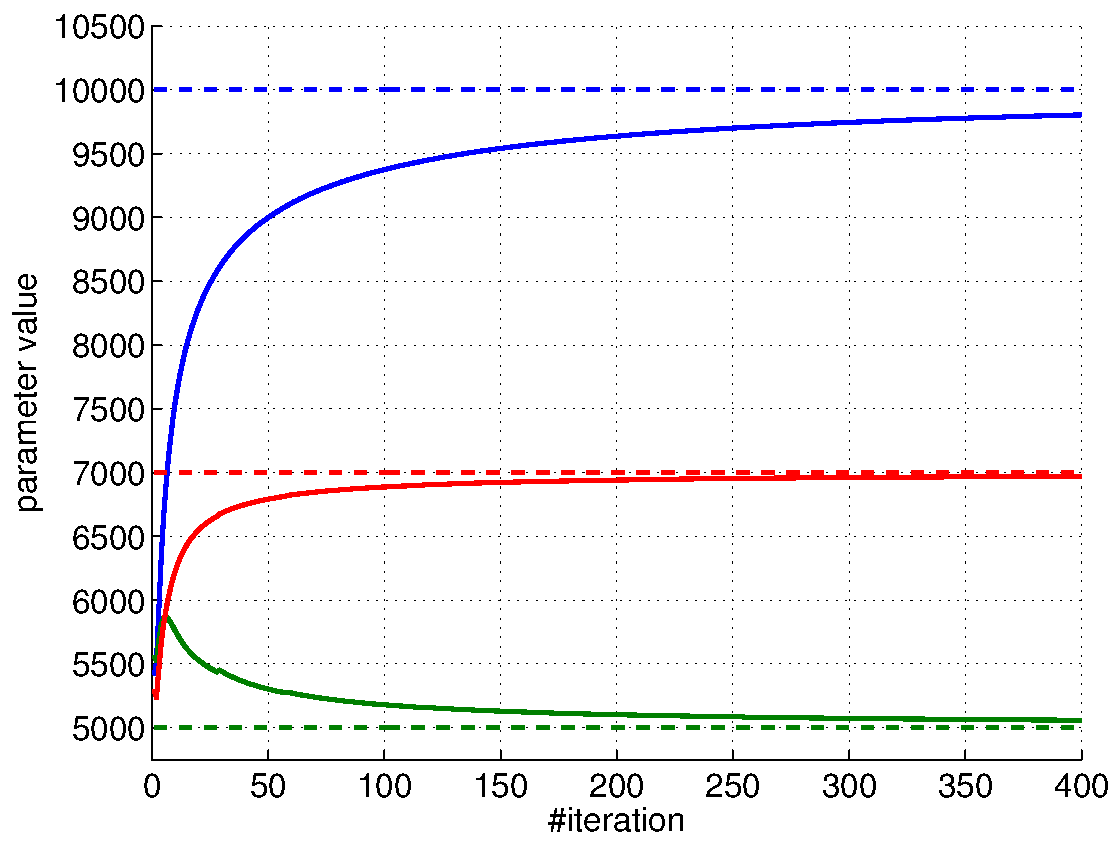
\includegraphics[width=.49\linewidth]{figures/p3_estim.pdf}
\hfill
%\subfigure[]{
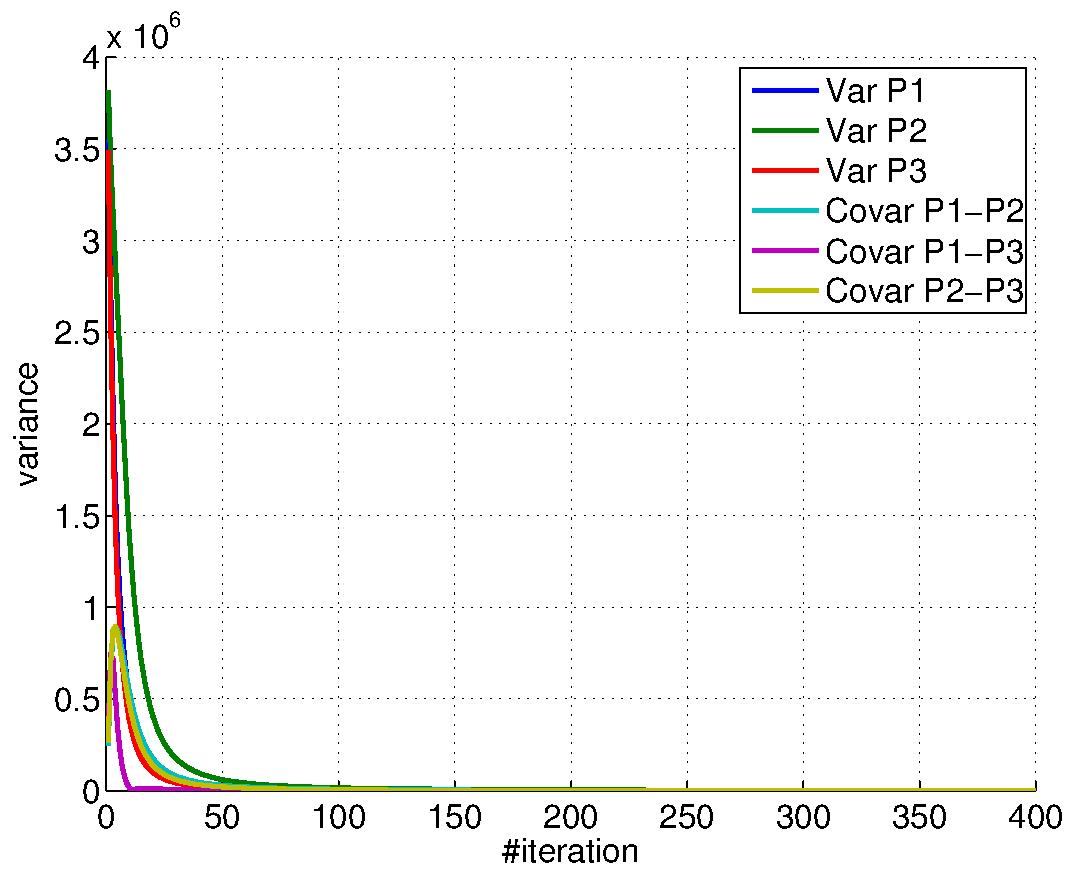
\includegraphics[width=.49\linewidth]{figures/p3_var.pdf}
\caption{Parameters: \texttt{initValue="6000"}, \texttt{stdev="2000"}. Observations: 10 points selected along the centerline,
\texttt{observationStdev=1e-3} no noise added. Although no noise added, we assume uncertainty of 1\,mm for each observation.}
\label{fig:Results3}
\end{center}
\end{figure}



\begin{figure}[ht]
\begin{center}
%\subfigure[]{
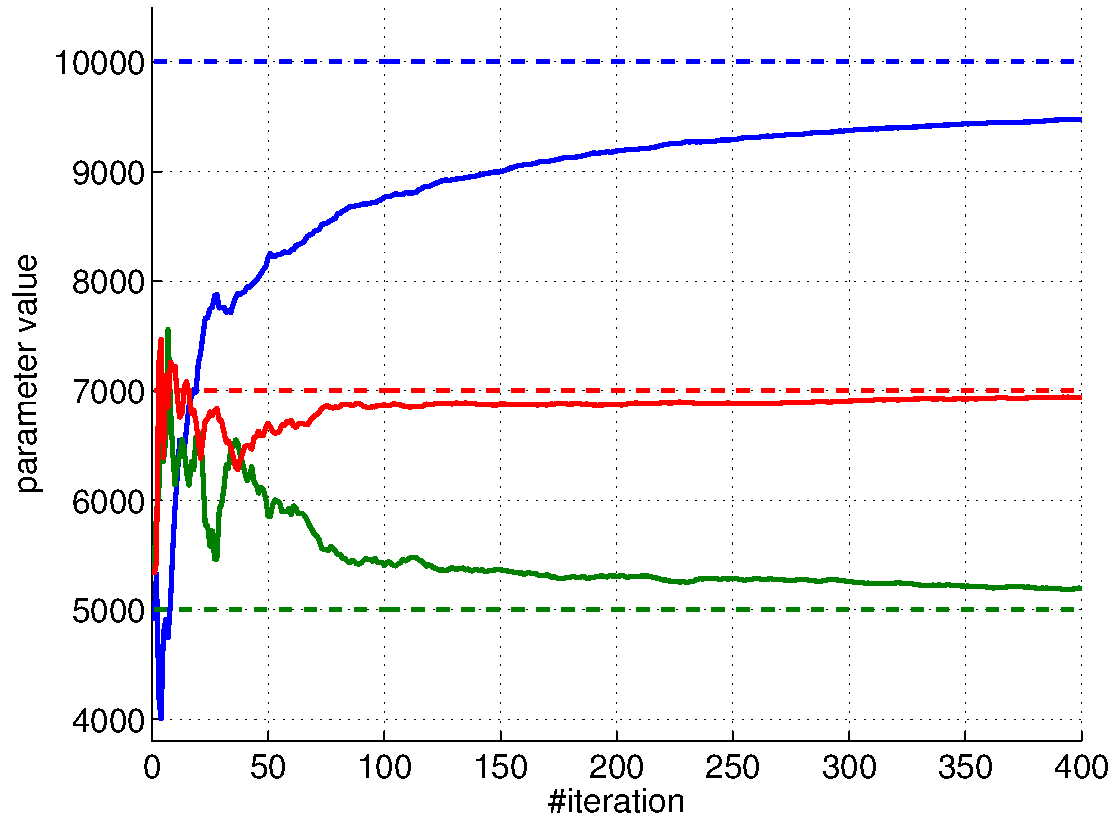
\includegraphics[width=.49\linewidth]{figures/p4_estim.pdf}
\hfill
%\subfigure[]{
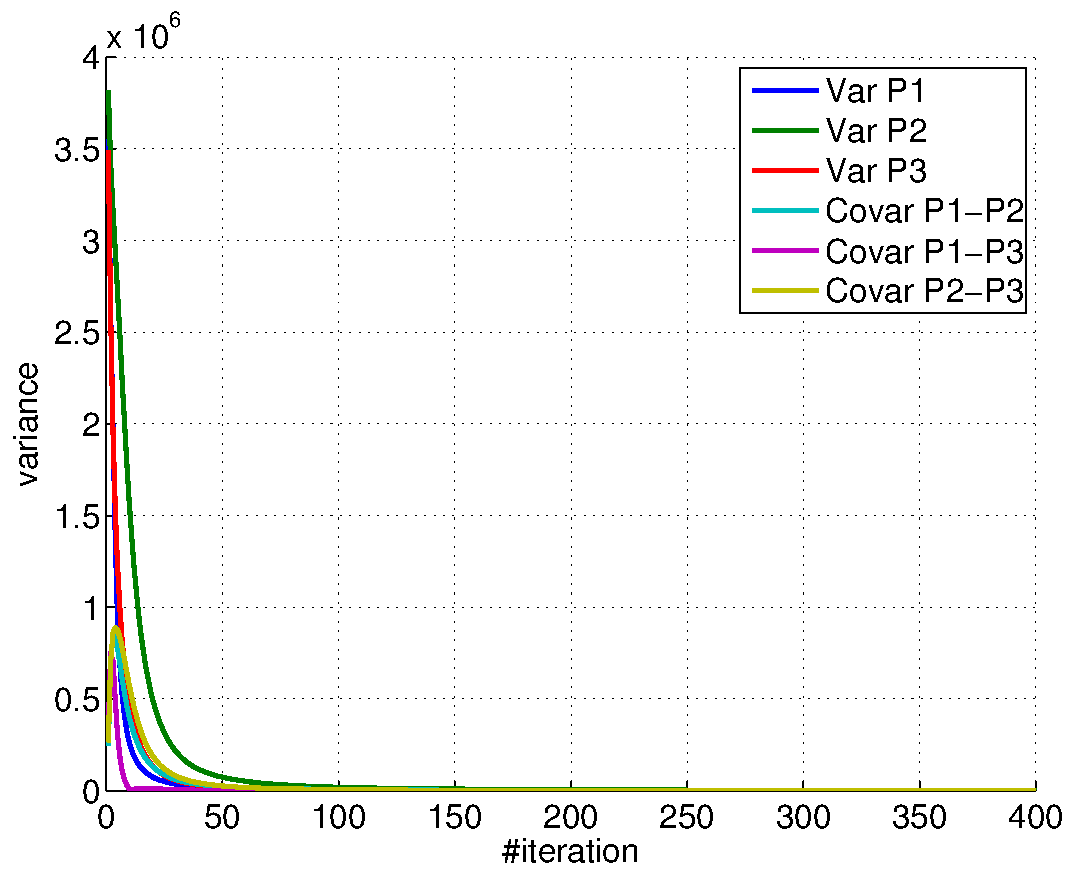
\includegraphics[width=.49\linewidth]{figures/p4_var.pdf}
\caption{Parameters: \texttt{initValue="6000"}, \texttt{stdev="2000"}. Observations: 10 points selected along the centerline,
\texttt{observationStdev=1e-3}, \texttt{noiseStdev=1e-3}. We have a real uncertainty of 1\,mm modeled with white Gaussian noise with standard
deviation of 1\,mm.}
\label{fig:Results4}
\end{center}
\end{figure}



\begin{figure}[ht]
\begin{center}
%\subfigure[]{
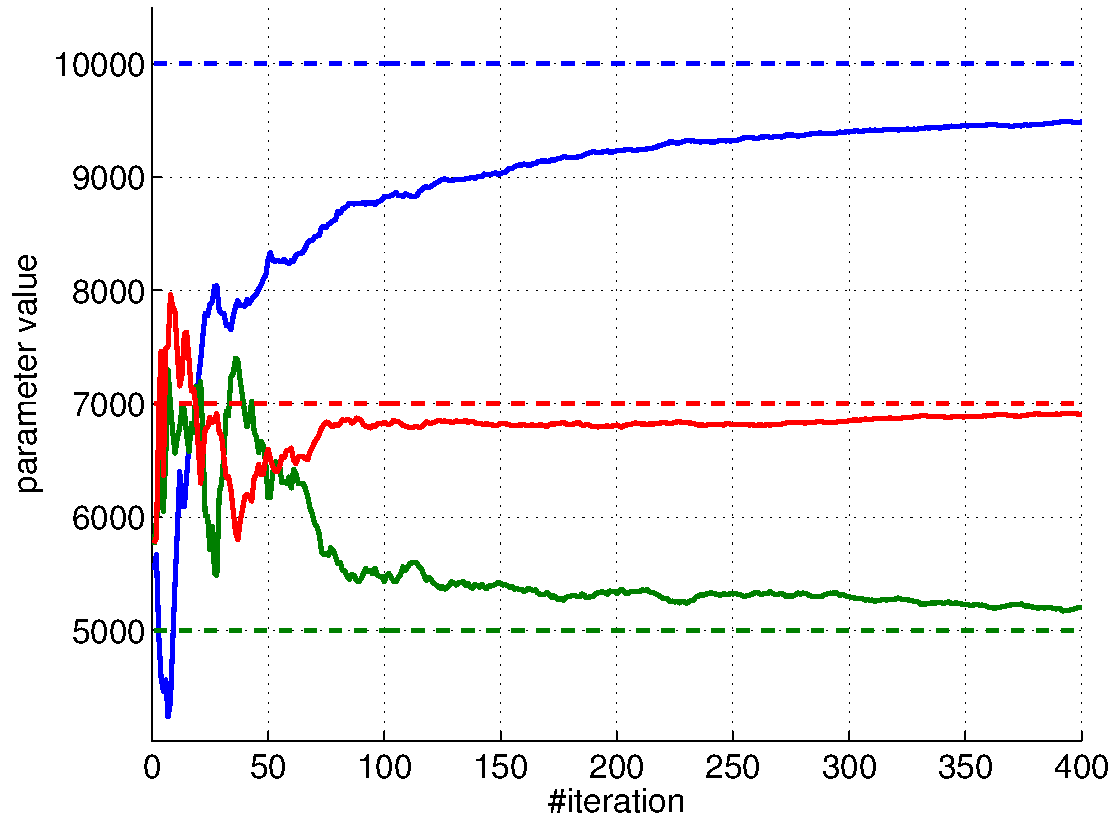
\includegraphics[width=.49\linewidth]{figures/p5_estim.pdf}
\hfill
%\subfigure[]{
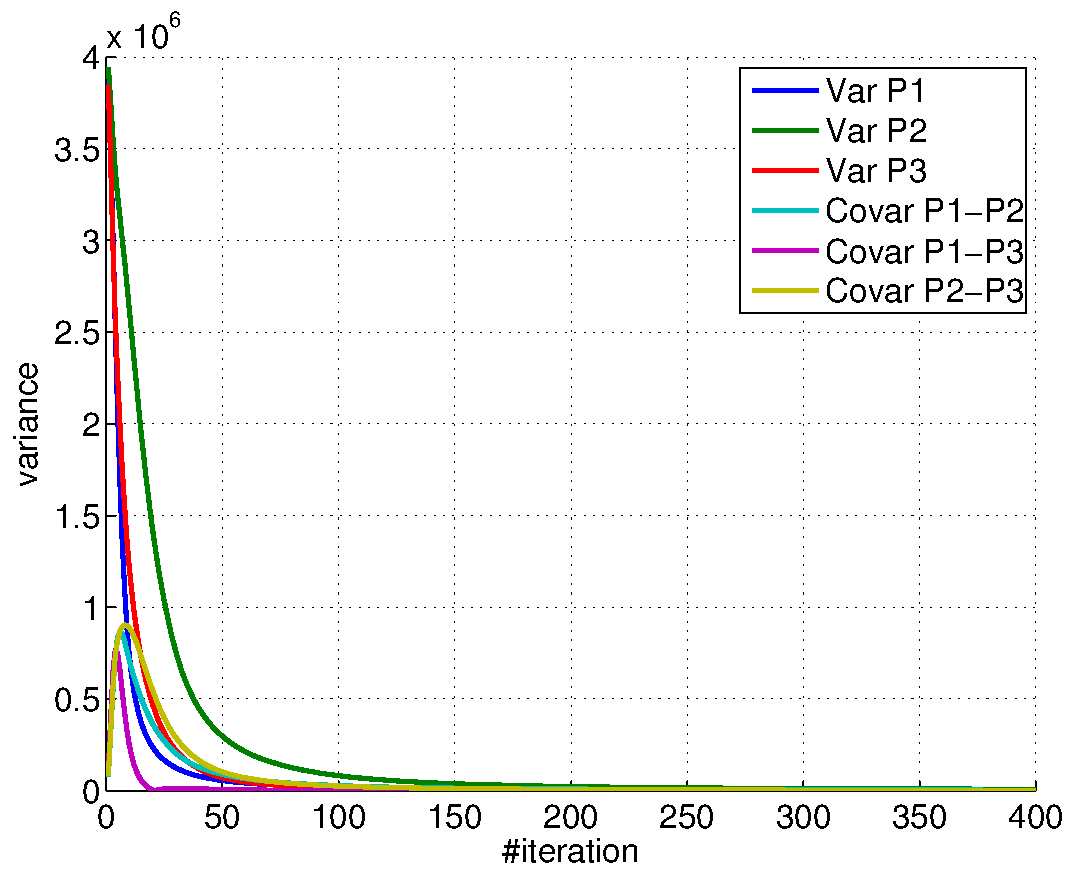
\includegraphics[width=.49\linewidth]{figures/p5_var.pdf}
\caption{Parameters: \texttt{initValue="6000"}, \texttt{stdev="2000"}. Observations: 10 points selected along the centerline,
\texttt{observationStdev=2e-3}, \texttt{noiseStdev=2e-3}. We have a real uncertainty of 2\,mm modeled with white Gaussian noise with standard
deviation of 2\,mm.}
\label{fig:Results5}
\end{center}
\end{figure}



\begin{figure}[ht]
\begin{center}
%\subfigure[]{
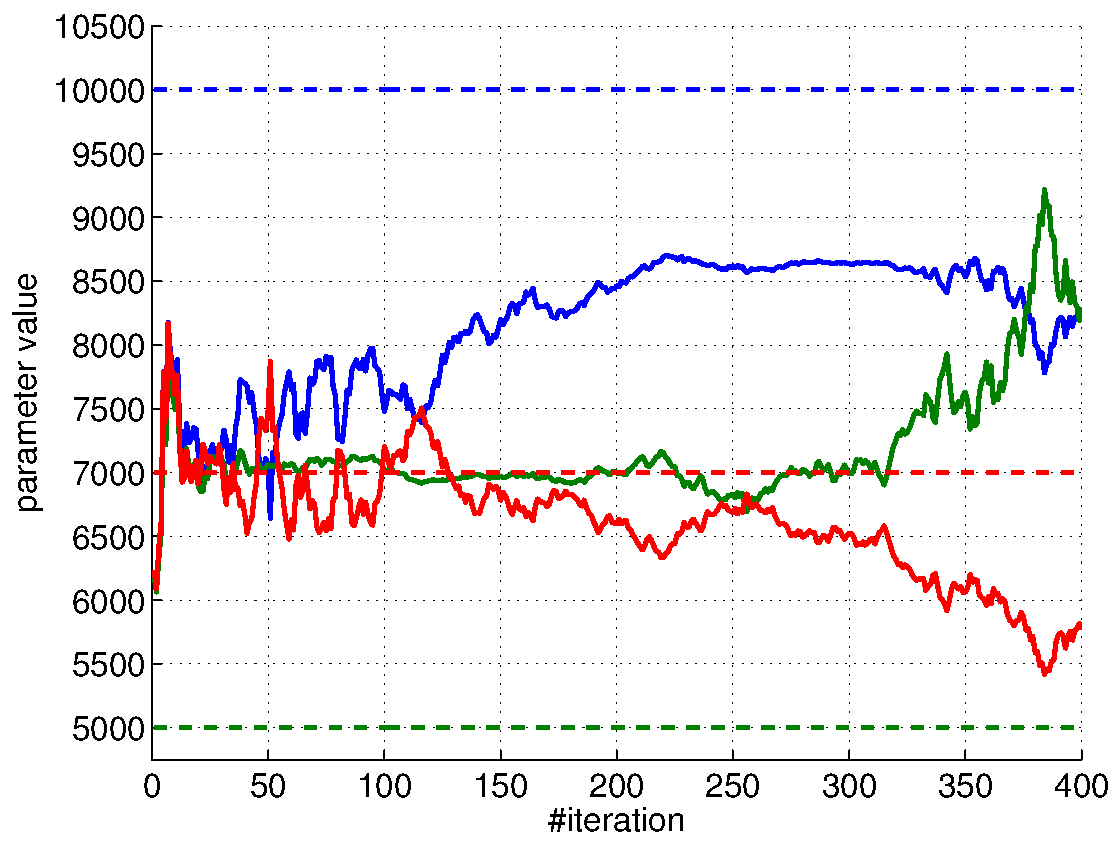
\includegraphics[width=.49\linewidth]{figures/p6_estim.pdf}
\hfill
%\subfigure[]{
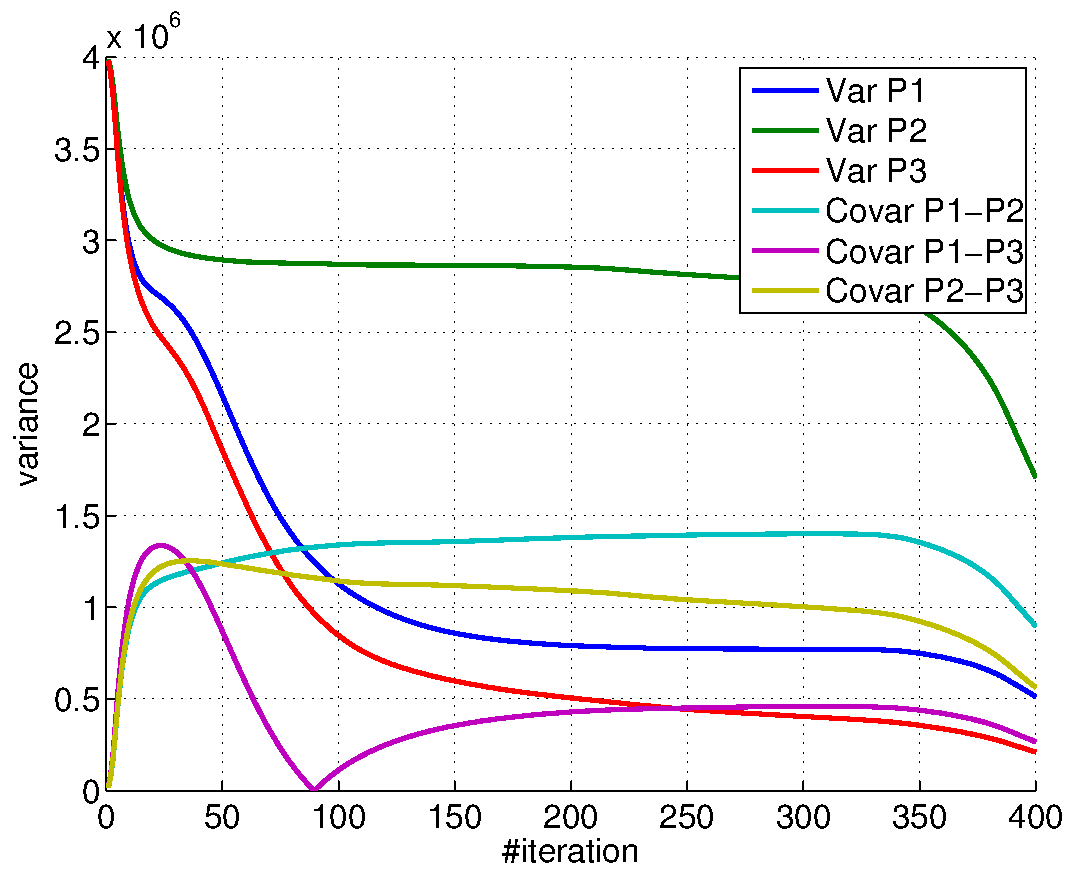
\includegraphics[width=.49\linewidth]{figures/p6_var.pdf}
\caption{Parameters: \texttt{initValue="6000"}, \texttt{stdev="2000"}. Observations: 1 point selected in the middle of the cylinder,
\texttt{observationStdev=2e-3}, \texttt{noiseStdev=2e-3}. An extreme case with fairly limited number of observations (a single point) and a real
uncertainty of 2\,mm modeled with white Gaussian noise with standard deviation of 2\,mm.}
\label{fig:Results6}
\end{center}
\end{figure}

\subsection{EX2: Estimation of varying Young's moduli of segements of a heterogeneous object under gravity}
The example is the same as the previous one, except for the fact that the Young's modulus is decreased from 6\,kPa to 2\,kPa between t=3\,s and t=5\,s.
The result is illustrated in figures (dash line is showing the value of parameters).

\begin{figure}[ht]
\begin{center}
%\subfigure[]{
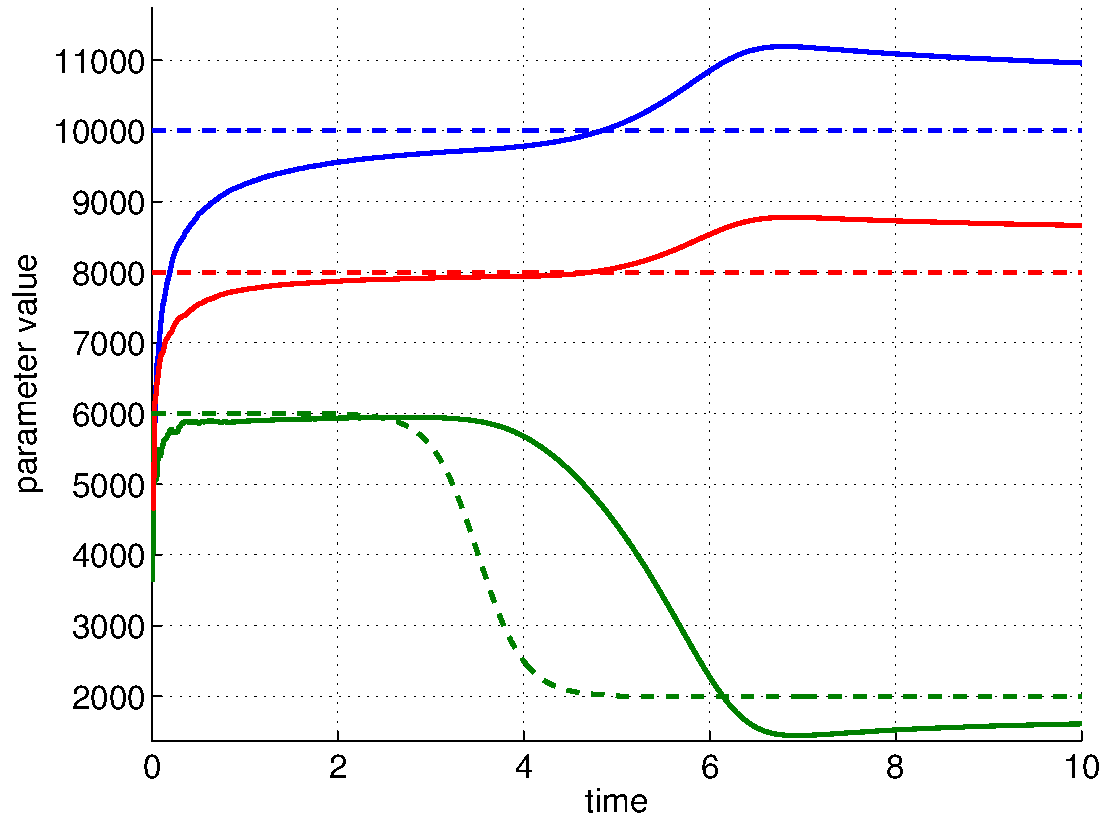
\includegraphics[width=.49\linewidth]{figures/pVarSm1_estim.pdf}
\hfill
%\subfigure[]{
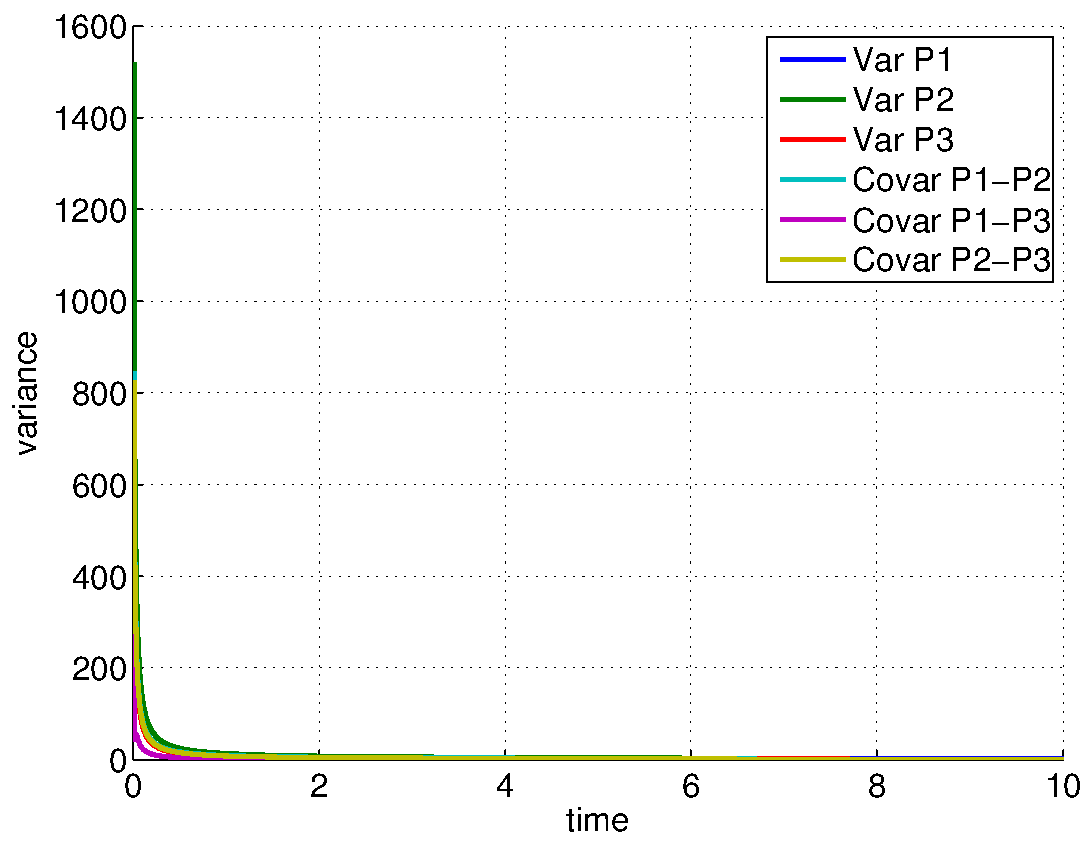
\includegraphics[width=.49\linewidth]{figures/pVarSm1_var.pdf}
\caption{Parameters: \texttt{initValue="6000"}, \texttt{stdev="2000"}. Observations: 10 points selected along the centerline,
\texttt{observationStdev=1e-4}, \texttt{noiseStdev=1e-4}. Even with no noise and very high confidence in measurement, the filter reacts to the 
change of the parameter with delay. Surprisingly, the other two parameters are perturbed as well.}
\label{fig:Results7}
\end{center}
\end{figure}

\begin{figure}[ht]
\begin{center}
%\subfigure[]{
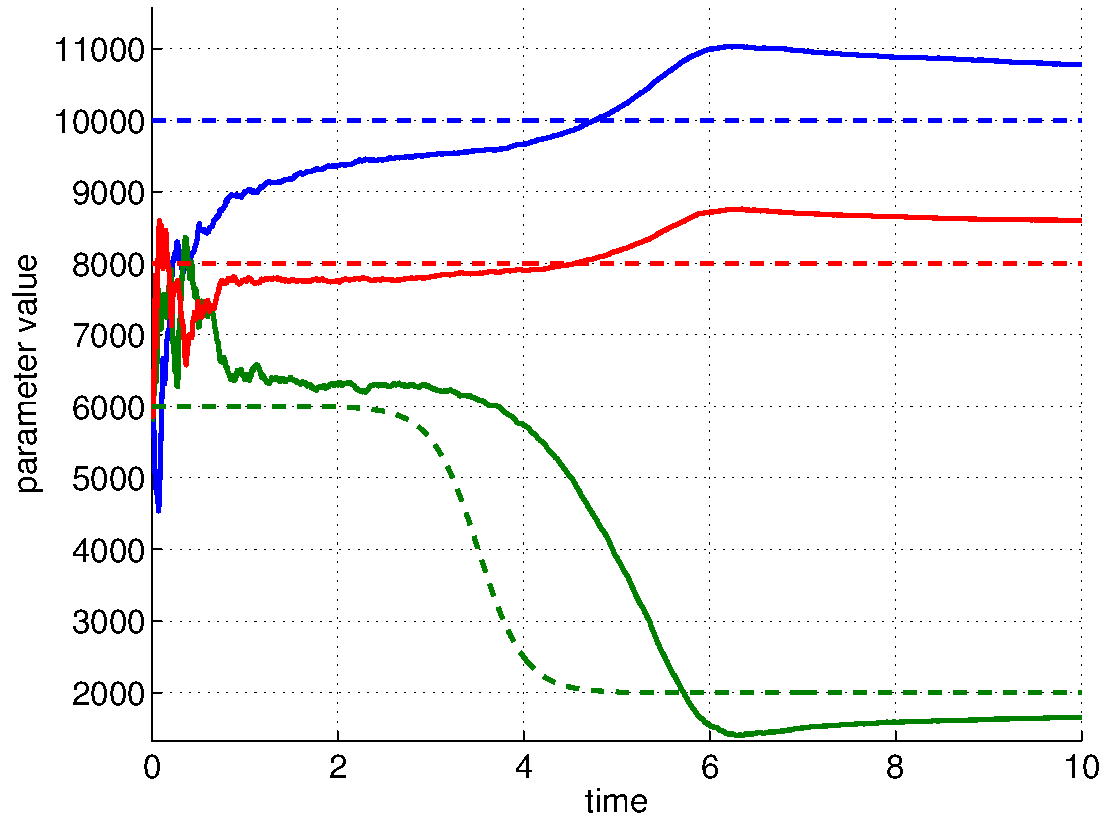
\includegraphics[width=.49\linewidth]{figures/pVarSm3_estim.pdf}
\hfill
%\subfigure[]{
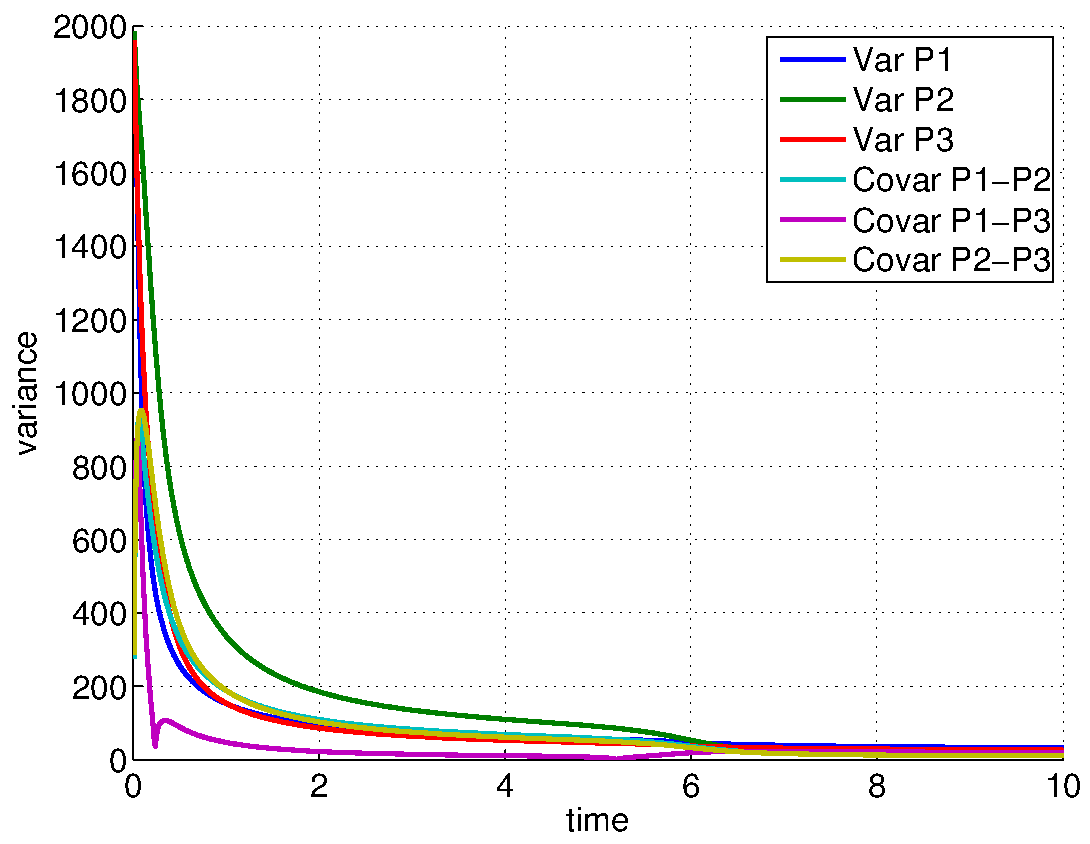
\includegraphics[width=.49\linewidth]{figures/pVarSm3_var.pdf}
\caption{Parameters: \texttt{initValue="6000"}, \texttt{stdev="2000"}. Observations: 10 points selected along the centerline,
\texttt{observationStdev=2e-3}, \texttt{noiseStdev=2e-3}. Despite the noise, the behavior of the filter is quite similar to the previous case when speaking about the adaptation of the 
varying parameter.}
\label{fig:Results8}
\end{center}
\end{figure}

\begin{figure}[ht]
\begin{center}
%\subfigure[]{
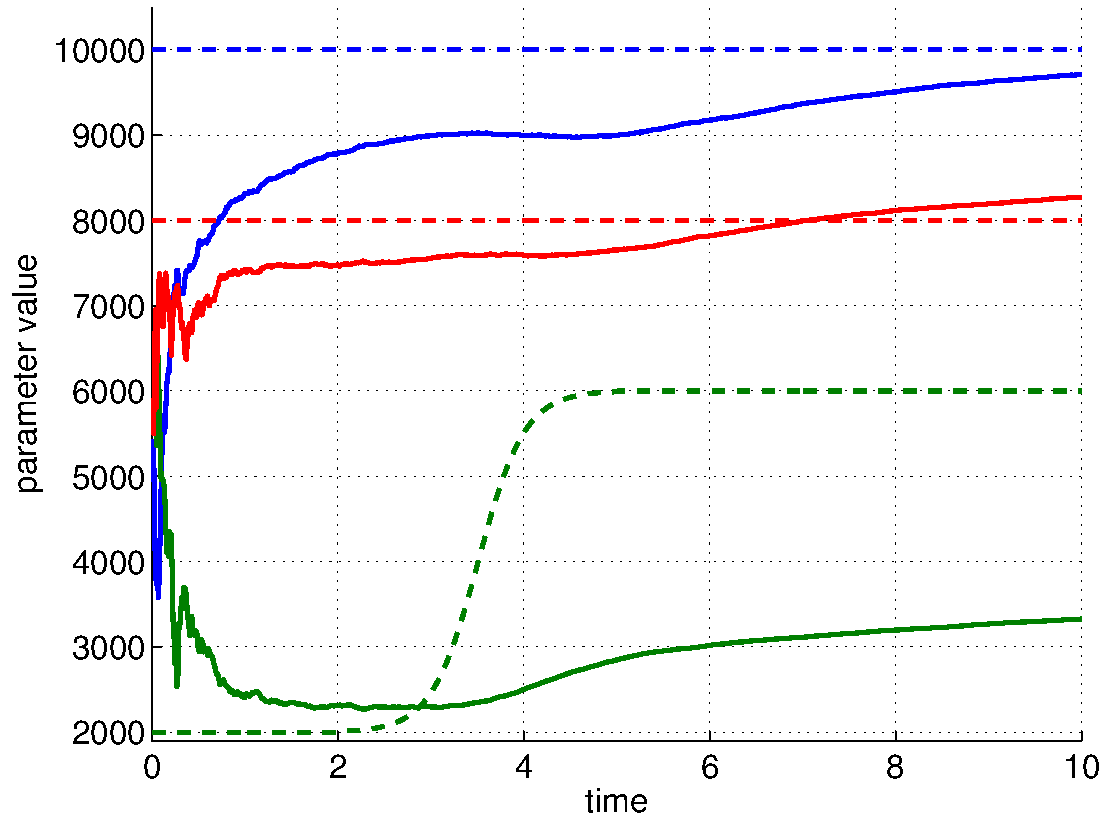
\includegraphics[width=.49\linewidth]{figures/pHardSmooth3_estim.pdf}
\hfill
%\subfigure[]{
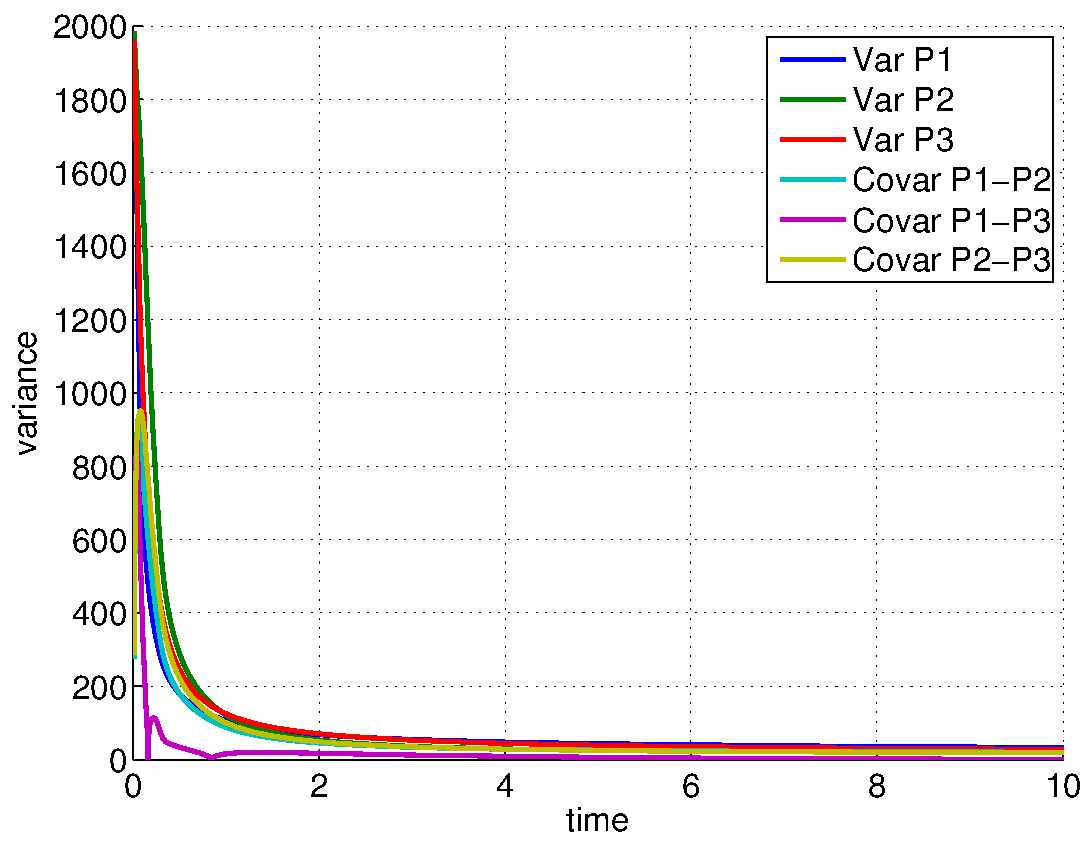
\includegraphics[width=.49\linewidth]{figures/pHardSmooth3_var.pdf}
\caption{Parameters: \texttt{initValue="6000"}, \texttt{stdev="2000"}. Observations: 10 points selected along the centerline,
\texttt{observationStdev=2e-3}, \texttt{noiseStdev=2e-3}, hardening instead of softening.
varying parameter.}
\label{fig:Results9}
\end{center}
\end{figure}


% \subsection{EX3: Estimation of a constant Young's modulus of each element of a heterogeneous object under gravity}
% In the forward simulation, the object is subject to gravity, while being composed of 3 segments, each having a different 
% Young's modulus ($E$) (10\,kPa, 2\,kPa, 8\,kPa). In the DA, the value of $E$ is treated as unknown independent coefficient for each element
% (\ie\ 770 parameters to be assimilated). The assimilation was tested for simplex and star $\sigma$-points.

% \begin{figure}[h]
% \begin{center}
% %\subfigure[]{
% \subfigure[]{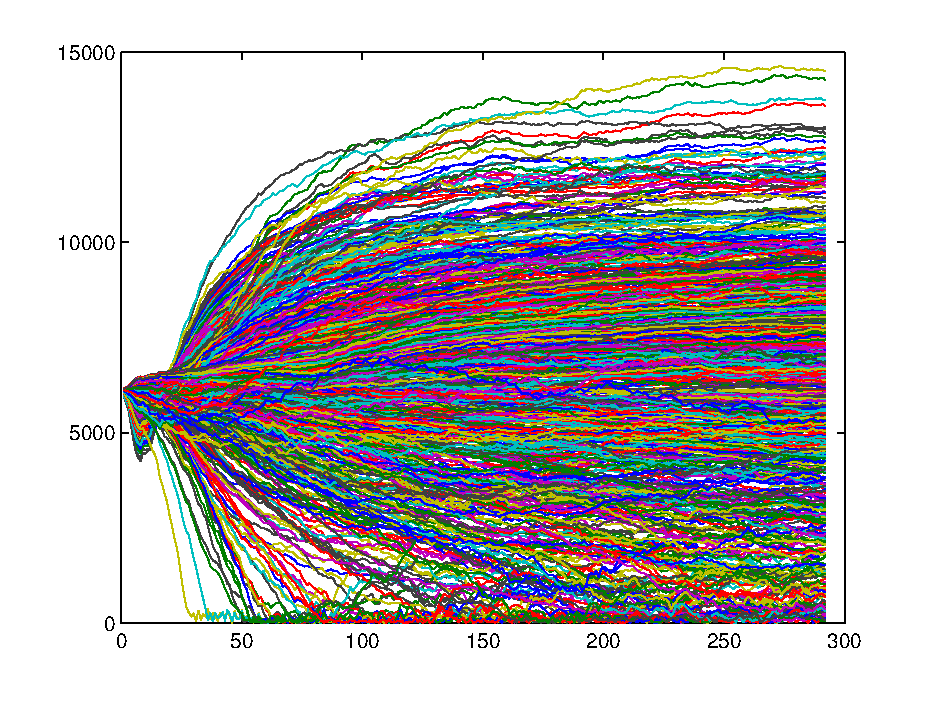
\includegraphics[width=.49\linewidth]{figures/cyl3AE_simplexAll.pdf}}
% \subfigure[]{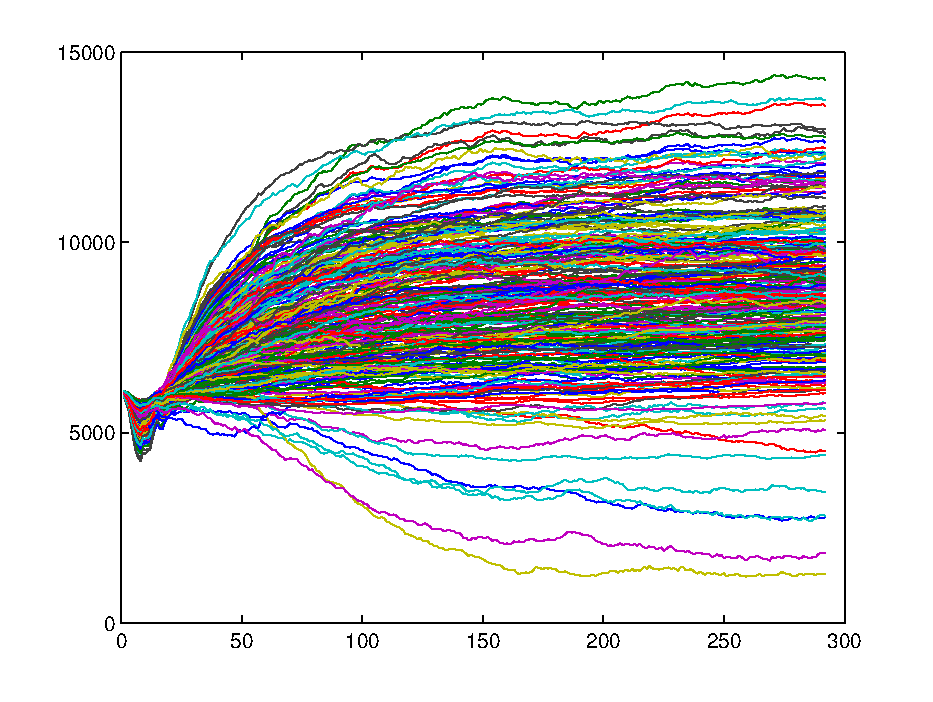
\includegraphics[width=.49\linewidth]{figures/cyl3AE_simplexS1.pdf}}
% \subfigure[]{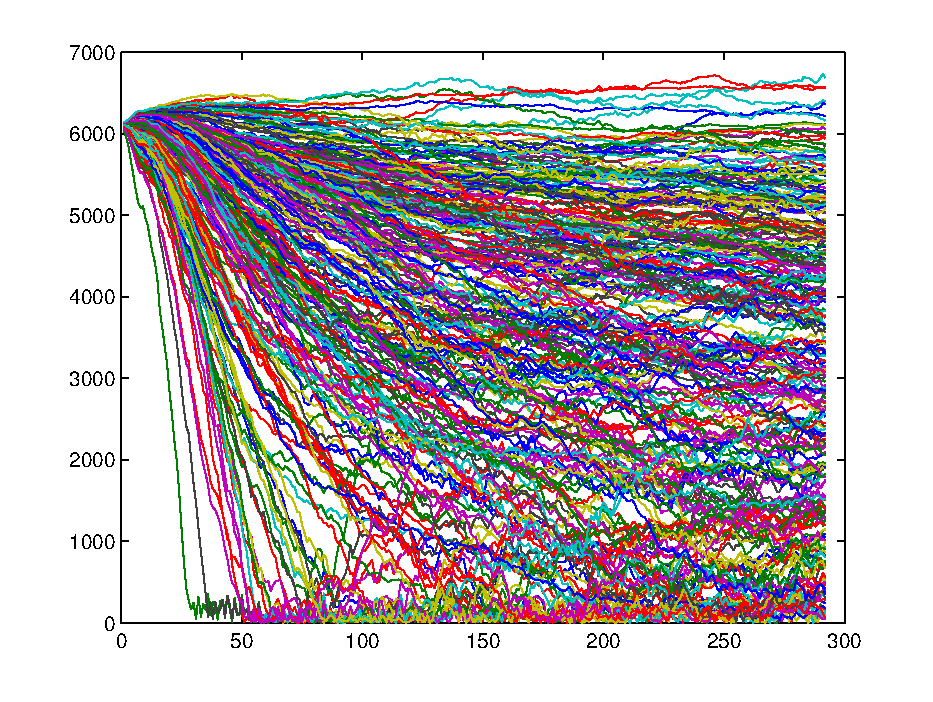
\includegraphics[width=.49\linewidth]{figures/cyl3AE_simplexS2.pdf}}
% \subfigure[]{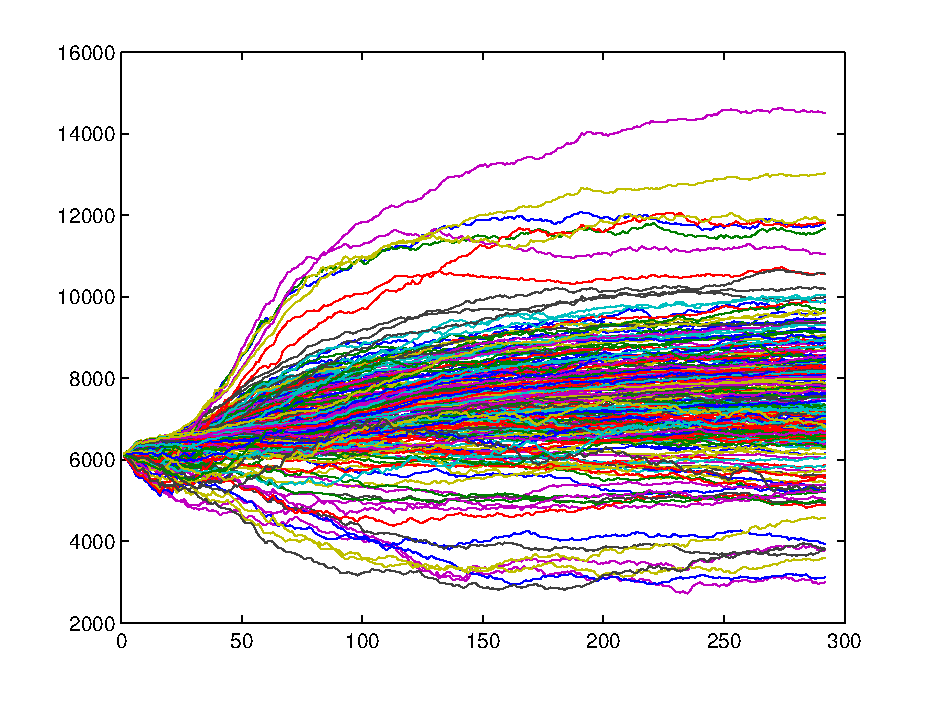
\includegraphics[width=.49\linewidth]{figures/cyl3AE_simplexS3.pdf}}
% \caption{Estimation of the constant $E$ for each element using {\bf simplex} $\sigma$-points: noise variance 0.002\,mm, using all degrees of freedom 
% as observations), assimilation executed for about 300 time steps (with dt=0.01s).
% (a) Assimilation of all the parameters; 
% (b) assimilation of parameters of elements beloning to segment 1 ($E_1$=10,000\,Pa, estimated mean: $\tilde{E}_1$ = 8,842\,Pa), 
% (c) segment 2 ($E_2$=2,000\,Pa, estimated mean: $\tilde{E}_2$ = 3,330\,Pa), 
% (d) segment 3 ($E_3$=8,000\,Pa, estimated mean: $\tilde{E}_1$ = 7,582\,Pa).}
% \label{fig:Results7}
% \end{center}
% \end{figure}

% \begin{figure}[h]
% \begin{center}
% %\subfigure[]{
% \subfigure[]{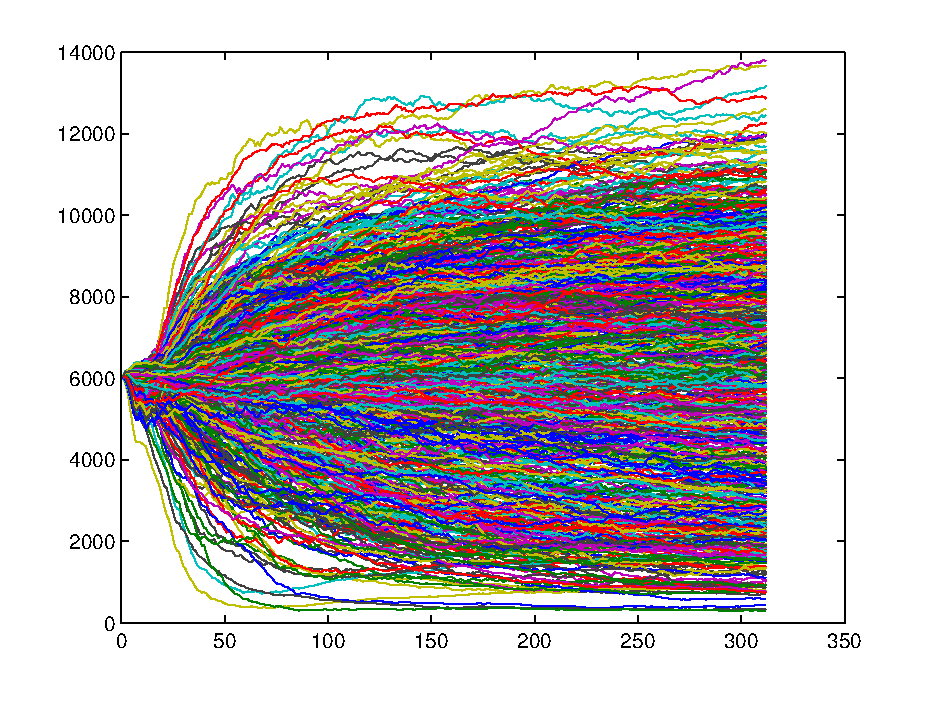
\includegraphics[width=.49\linewidth]{figures/cyl3AE_starAll.pdf}}
% \subfigure[]{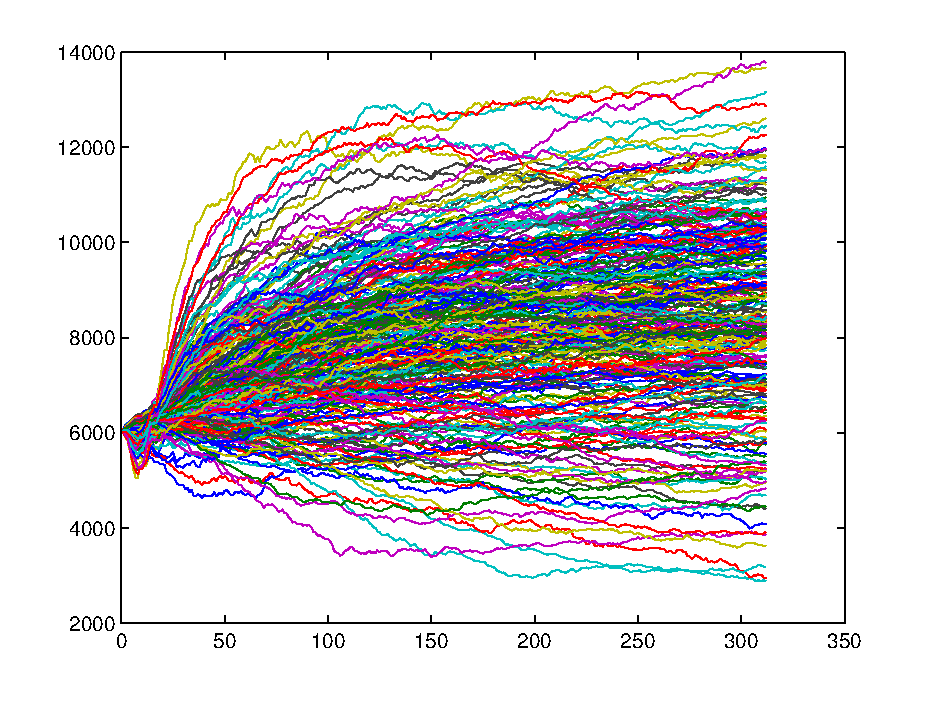
\includegraphics[width=.49\linewidth]{figures/cyl3AE_starS1.pdf}}
% \subfigure[]{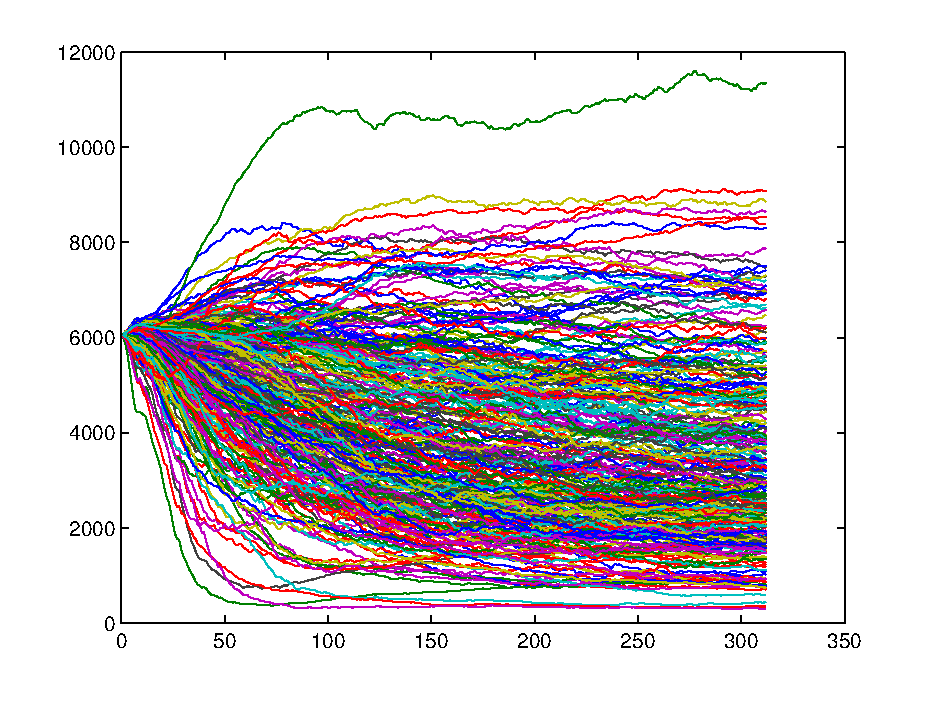
\includegraphics[width=.49\linewidth]{figures/cyl3AE_starS2.pdf}}
% \subfigure[]{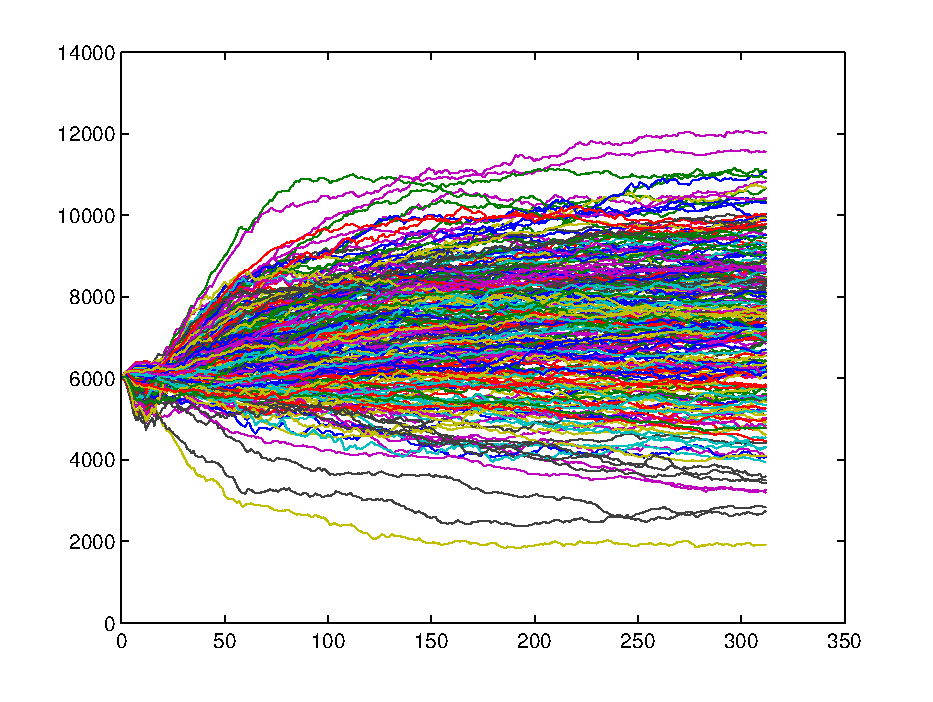
\includegraphics[width=.49\linewidth]{figures/cyl3AE_starS3.pdf}}
% \caption{Estimation of the constant $E$ for each element using {\bf star} $\sigma$-points: noise variance 0.002\,mm, using all degrees of freedom 
% as observations), assimilation executed for about 300 time steps (with dt=0.01s).
% (a) Assimilation of all the parameters; 
% (b) assimilation of parameters of elements beloning to segment 1 ($E_1$=10,000\,Pa, estimated mean: $\tilde{E}_1$ = 8,515\,Pa), 
% (c) segment 2 ($E_2$=2,000\,Pa, estimated mean: $\tilde{E}_2$ = 3,487\,Pa), 
% (d) segment 3 ($E_3$=8,000\,Pa, estimated mean: $\tilde{E}_1$ = 7,394\,Pa).}
% \label{fig:Results7}
% \end{center}
% \end{figure}


\section{Notes}

\subsection{Static vs. Dynamic}
The graphs in the EX1 were obtained using quasi-static scenario, \ie\ \texttt{StaticSolver} having \texttt{applyIncrementFactor="1"}. Observations:
\begin{itemize}
 \item The result with the \texttt{StaticSolver} depend on \texttt{dt}: the results were obtained with \texttt{dt=0.01s}. Comparable results can be
achieved with \texttt{dt=0.1}, 
 the \ssda\ remains stable even for dt of 1\,s.
 \item The stability of the \ssda\ seems to depend on the integration scheme, as with \texttt{EulerImplicitSolver} the method seems to be less stable.
The stability depends on \texttt{Rayleigh stiffness}: a behavior comparable to the static behavior is achieved with RS=0.5, the process is stable and
the final approximation is even more precise that in the static case. 
\item With decreasing RS, the DA becomes less stable in the beginning since the change in positions is too fast and so the perturbations becomes
``wild''. 
\end{itemize}


\bibliographystyle{unsrt}
\bibliography{references}


\end{document}
